\documentclass[12pt]{ctexart}
\usepackage{amsmath, amsthm, amssymb, bm, graphicx, hyperref, mathrsfs, cite, subcaption, geometry}

\title{\textbf{基因编辑技术在疾病诊疗中的应用}}
\author{凌星皓\\化学系 \space 课程论文}
\linespread{1.5}

\newtheorem{theorem}{定理}[section]
\newtheorem{definition}[theorem]{定义}
\newtheorem{lemma}[theorem]{引理}
\newtheorem{corollary}[theorem]{推论}
\newtheorem{example}[theorem]{例}
\newtheorem{proposition}[theorem]{命题}
\renewcommand{\abstractname}{\Large\textbf{摘要}}
\captionsetup{margin=18pt, font=small}
\pagestyle{plain}
\geometry{a4paper,scale=0.75}
\hypersetup
    {
        hypertex=true,
        colorlinks=true,
        linkcolor=blue,
        anchorcolor=blue,
        citecolor=blue
    }%超链接


\begin{document}

\maketitle
% \setcounter{page}{0}

\begin{abstract}
    回顾了基因编辑技术的基本内容和原理，并实例性地描述了其在基因缺陷、CAR-T治疗中的应用。
    \par\textbf{关键词：}基因编辑，CRISPR/Cas-9，CAR-T，基因缺陷
\end{abstract}

\section{引言}
基因编辑技术是一种基于对DNA序列的特异性识别与操作所构造的生物技术。最初对修改基因的尝试来自限制性核酸内切酶，当其成功在特定位点切割dsDNA后，细胞内的同源重组(HR)和非同源末端连接(NHEJ)等修复机制被增强\cite{capecchiAlteringGenomeHomologous1989}。从细胞的角度来说，DNA一旦被破坏而未能修复，那么整段编码蛋白的DNA就会成为错误编码而被缄默，这对于基因组和蛋白功能的研究具有重要的价值。
\par 在上述思路中，精确定位目标的基因是关键问题。研究者们陆续提出基于MegNs, ZFN, TALEN, CRISPER/Cas9基因编辑技术\cite{khalilGenomeEditingRevolution2020}。其共同点是由识别体和内切酶两部分构成。ZFN和TALEN技术基于蛋白质三维构象对特定碱基的识别；而CRISPER/Cas9技术(图\ref{crispr})则基于Cas9蛋白和向导RNA的复合体，大大减小了切割的脱靶率。后者通过设计\textbf{sgRNA序列}即可令该体系根据互补识别在特定位点切开DNA(Double Strand Break, DSB)，因而成为流行且方便的基因编辑技术，并基于该技术发展出荧光示踪、促转录、抑制转录等多种相关功能。
\begin{figure}[h] 
    \centering
    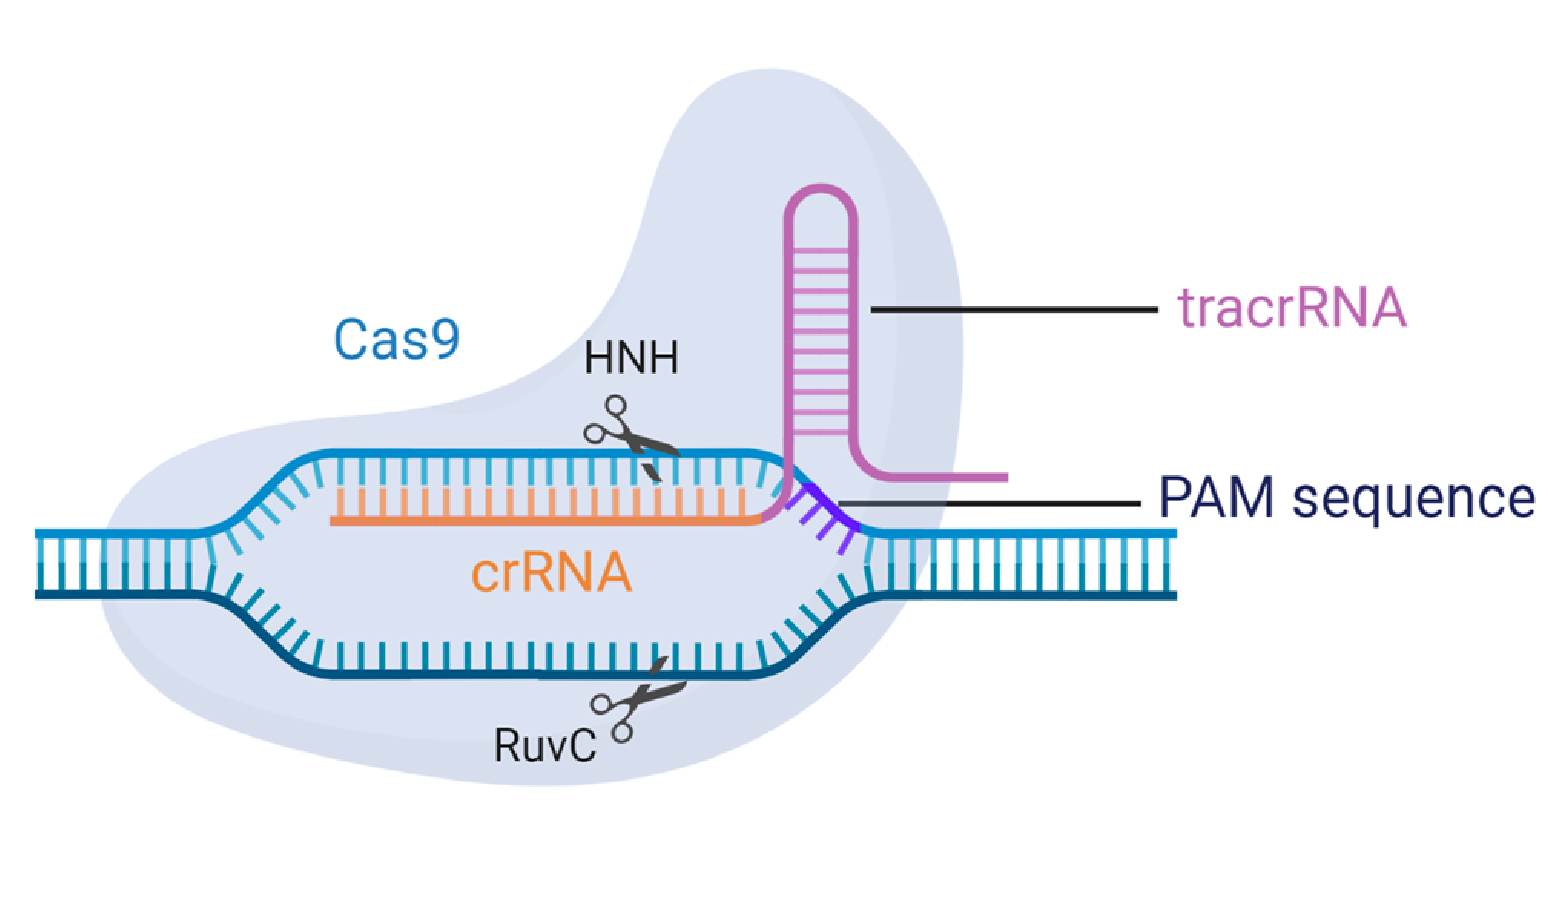
\includegraphics[width=0.7\textwidth]{crispr.png}
    \caption{CRISPER/Cas9 system\qquad sgRNA由crRNA和tracrRNA组成，后者能结合Cas9蛋白形成复合物。Cas9蛋白会先识别和牵引PAM区(protospacer adjacent motif)，其由任意5‘-NGG序列构成；后根据sgRNA比对上游的DNA，并由内切酶对目标DNA切割。该机制最先在细菌中作为一种适应性免疫应答被发现。}
    \label{crispr}
\end{figure}
\par 基因编辑技术的发展为疾病诊疗提供了新的技术和思路，本文将在遗传性疾病和恶性肿瘤的治疗中各选一例进行梳理，以展现其巨大的潜力。
\section{基因编辑技术用于基因缺陷的矫正}
基因编辑技术特异性地调控基因序列的能力让矫正遗传性疾病成为可能。2017年，研究者们\cite{maCorrectionPathogenicGene2017}通过CRISPR/Cas-9技术成功矫正了遗传肥厚性心肌病(hypertrophic cardiomyopathy,HCM)，一种因晚发性而避免自然选择、发病率较高的遗传疾病。其发病被认为与常染色体上MYBPC3基因的显性突变有关。从基因编辑的角度来看，在切割基因后，前述NHEJ机制会导致缄默和基因改变，而另一种修复机制(即同源介导的修复,HDR)利用核内存在的同源片段为模版修复受损DNA，被认为具有修复胚胎基因缺陷的潜力。
\par 为了确认该机制在人类细胞中的效率，研究者使用一名遗传性HCM男性患者的组织样本培养诱导性多能干细胞 (iPSCs)，其在MYBP3基因的外显子16段有一个4碱基的缺失突变。向导RNA(sgRNA)被设计为靶向该基因区域，寡廉核苷酸(ssODN)模版则被设计为具有为同源臂和同义突变(synonymous substitution)。表达Cas9蛋白和上述核酸序列的质粒一同经电转染入iPSC细胞，克隆的细胞经测序分析其效果。其中插入缺失标记(inDel)者为成功切割并经过NHEJ修复、同义突变者即经过HDR修复机制。由此研究者证明CRISPR/Cas9可以靶向突变位点，说明了该技术的可行性。
\begin{figure}[h] 
    \centering
    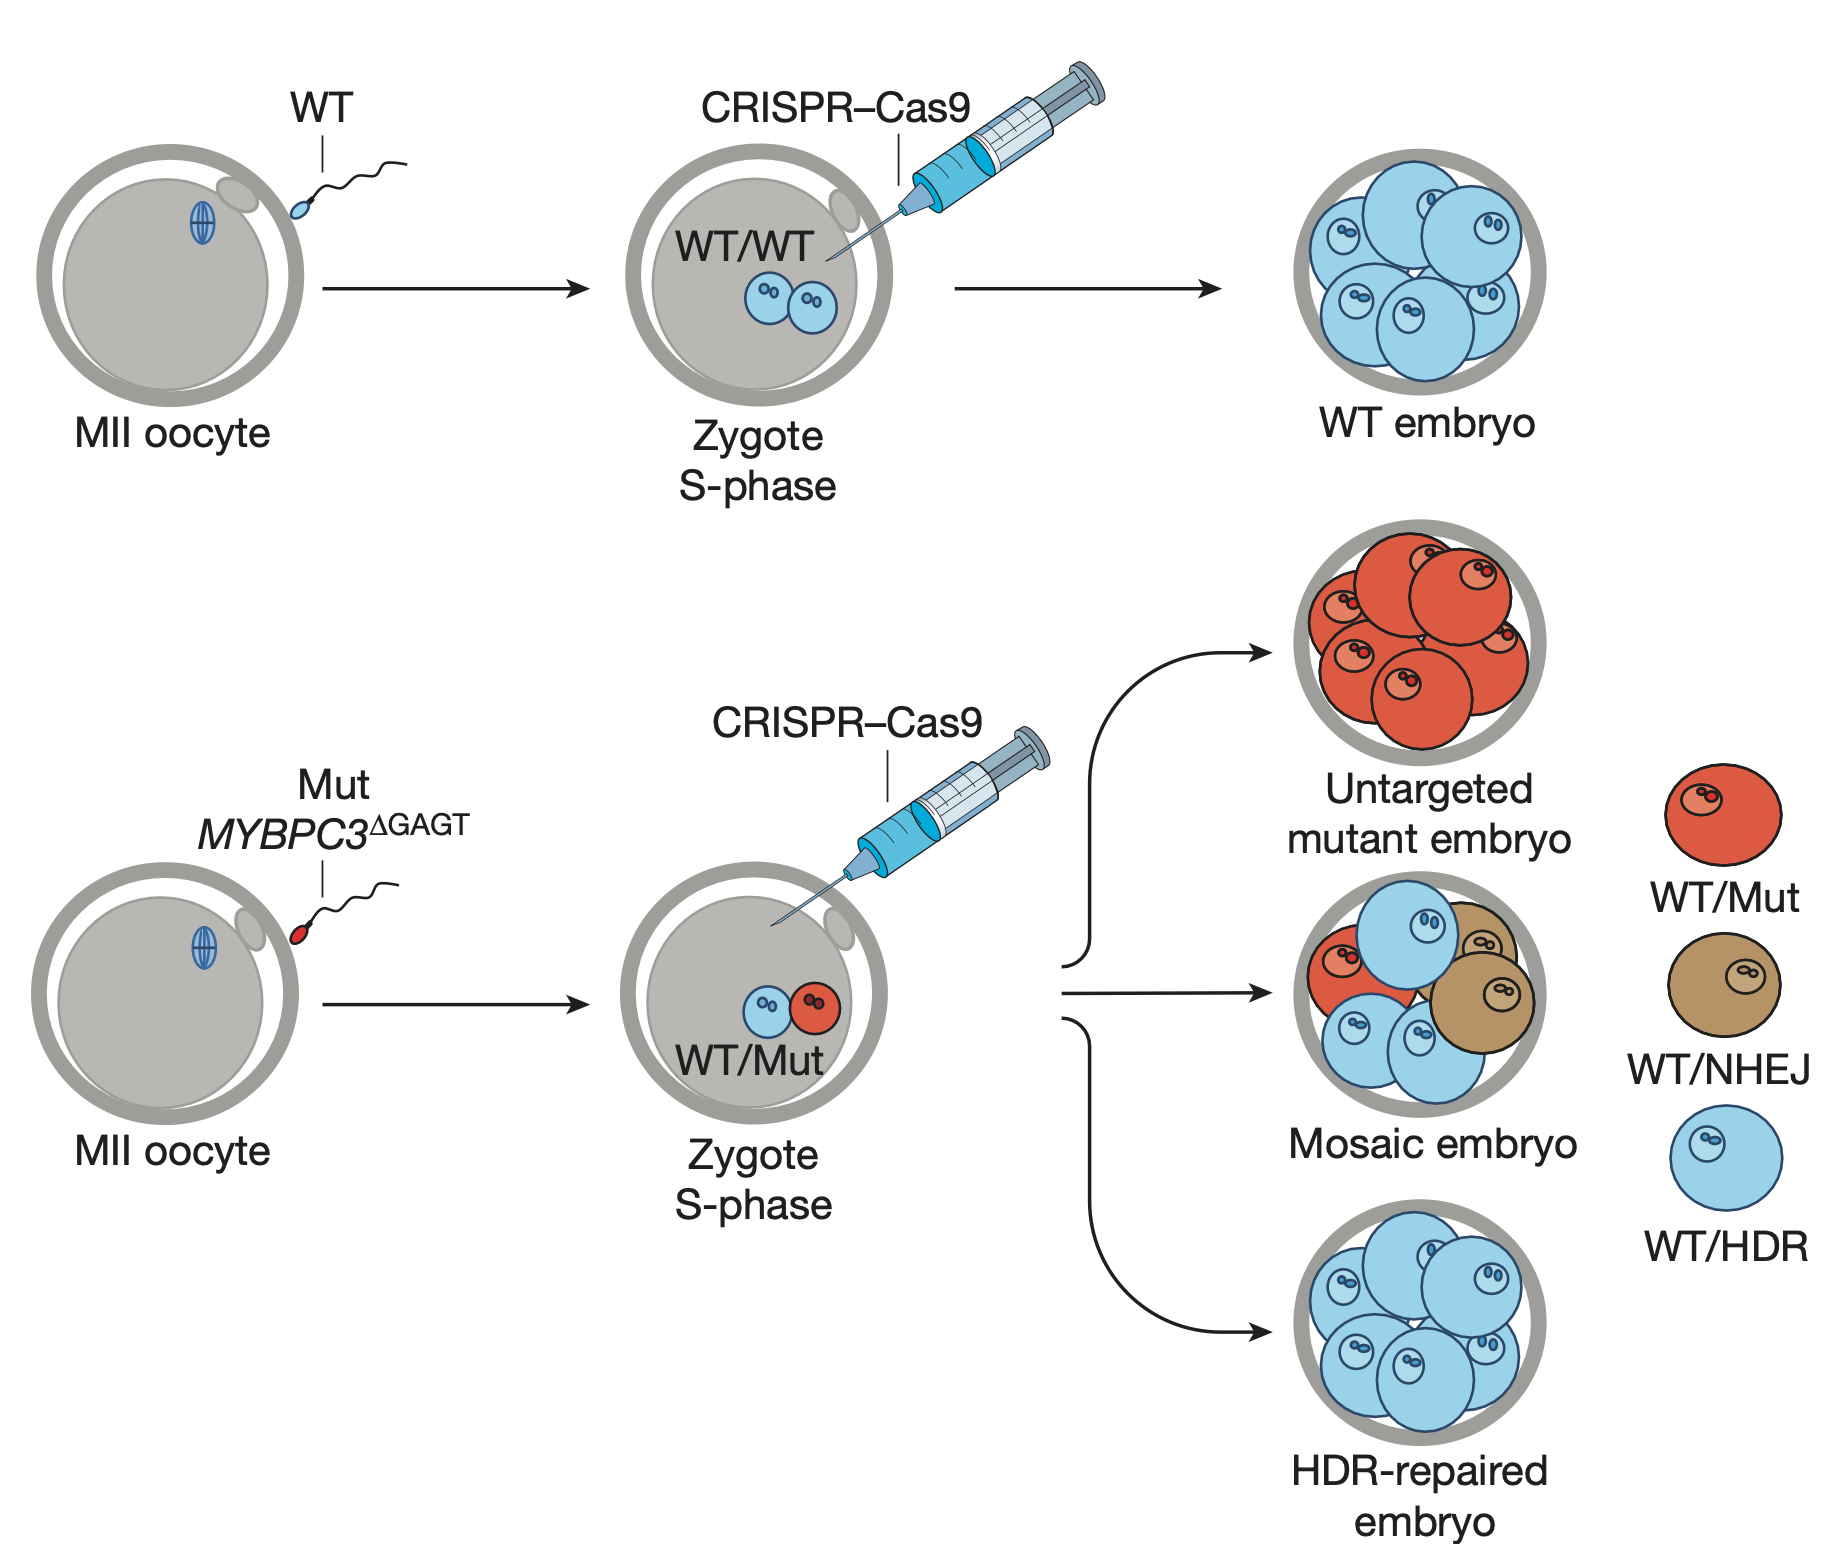
\includegraphics[width=0.7\textwidth]{sjl.png}
    \caption{S-phase注射的人体胚胎细胞基因矫正}
    \label{sjl}
\end{figure}
\par 随后，研究者将显性突变的精子同健康的卵母细胞孵育，并在18小时后将上述设计的Cas9蛋白、sgRNA、ssODN DNA直接注射进入原核期受精卵的胞浆中(图\ref{sjl})。经过多个受精卵的分析和对照实验，研究者认为受精卵中的基因编辑具有较高的靶向效率。其后，为了检查脱靶效应，研究者在全基因组测序后，对23个可能是脱靶的位点进行了更仔细的分析，确认了其未在任何非靶向位点造成变化。
\par 这项研究表明通过基因剪切后激活HDR修复的途径具有基因矫正治疗的潜力，尽管仍面临体细胞中HDR修复效率低和修复机理不明晰等问题。目前，基于基因编辑的技术已经用于其他一些遗传疾病的治疗，包括转甲状腺素蛋白心脏淀粉样变(ATTR)\cite{gillmoreCRISPRCas9VivoGene2021}和镰刀型红血球疾病(SCD)\cite{frangoulCRISPRCas9GeneEditing2021}等。值得讨论的一点在于，若非对胚胎进行基因编辑，那就意味着需要对某一特别的细胞进行功能改造(不可能对所有细胞都改造)，也就势必需要高效的\textbf{递送体系}将Cas9蛋白运送到靶向的细胞内，以增加或减少某种蛋白的合成和表达。概括来说，该系统需要完成封装和递送两个任务，以令基因编辑体系仅在病灶处生效。譬如使用温度敏感的水凝胶靶向肿瘤细胞、脂质纳米颗粒靶向肝细胞等。
\section{基因编辑技术用于Car-T疗法}
\par 上节讨论了\textbf{遗传类疾病}中通过基因编辑治疗的思路，实际上该技术也广泛用于其他的新兴治疗方法。其中，CAR-T(Chimeric Antigen Receptor T-cells)疗法近年来的发展为血液癌患者带来了希望\cite{dimitriEngineeringNextgenerationCAR2022}。该方法由桑名义久(Yoshihisa Kuwana)等人首次描述，通过将靶向癌细胞的抗体结构域同T细胞表面的激活受体嵌合，使得T细胞被改造而能够\textbf{特异性}摧毁癌细胞(图\ref{cart})。实际治疗中，T细胞常从患者本人血液中分离并进行基因改造(如通过病毒载体插入嵌合受体的基因)，令其能够表达上述嵌合受体。
\begin{figure}[h] 
    \centering
    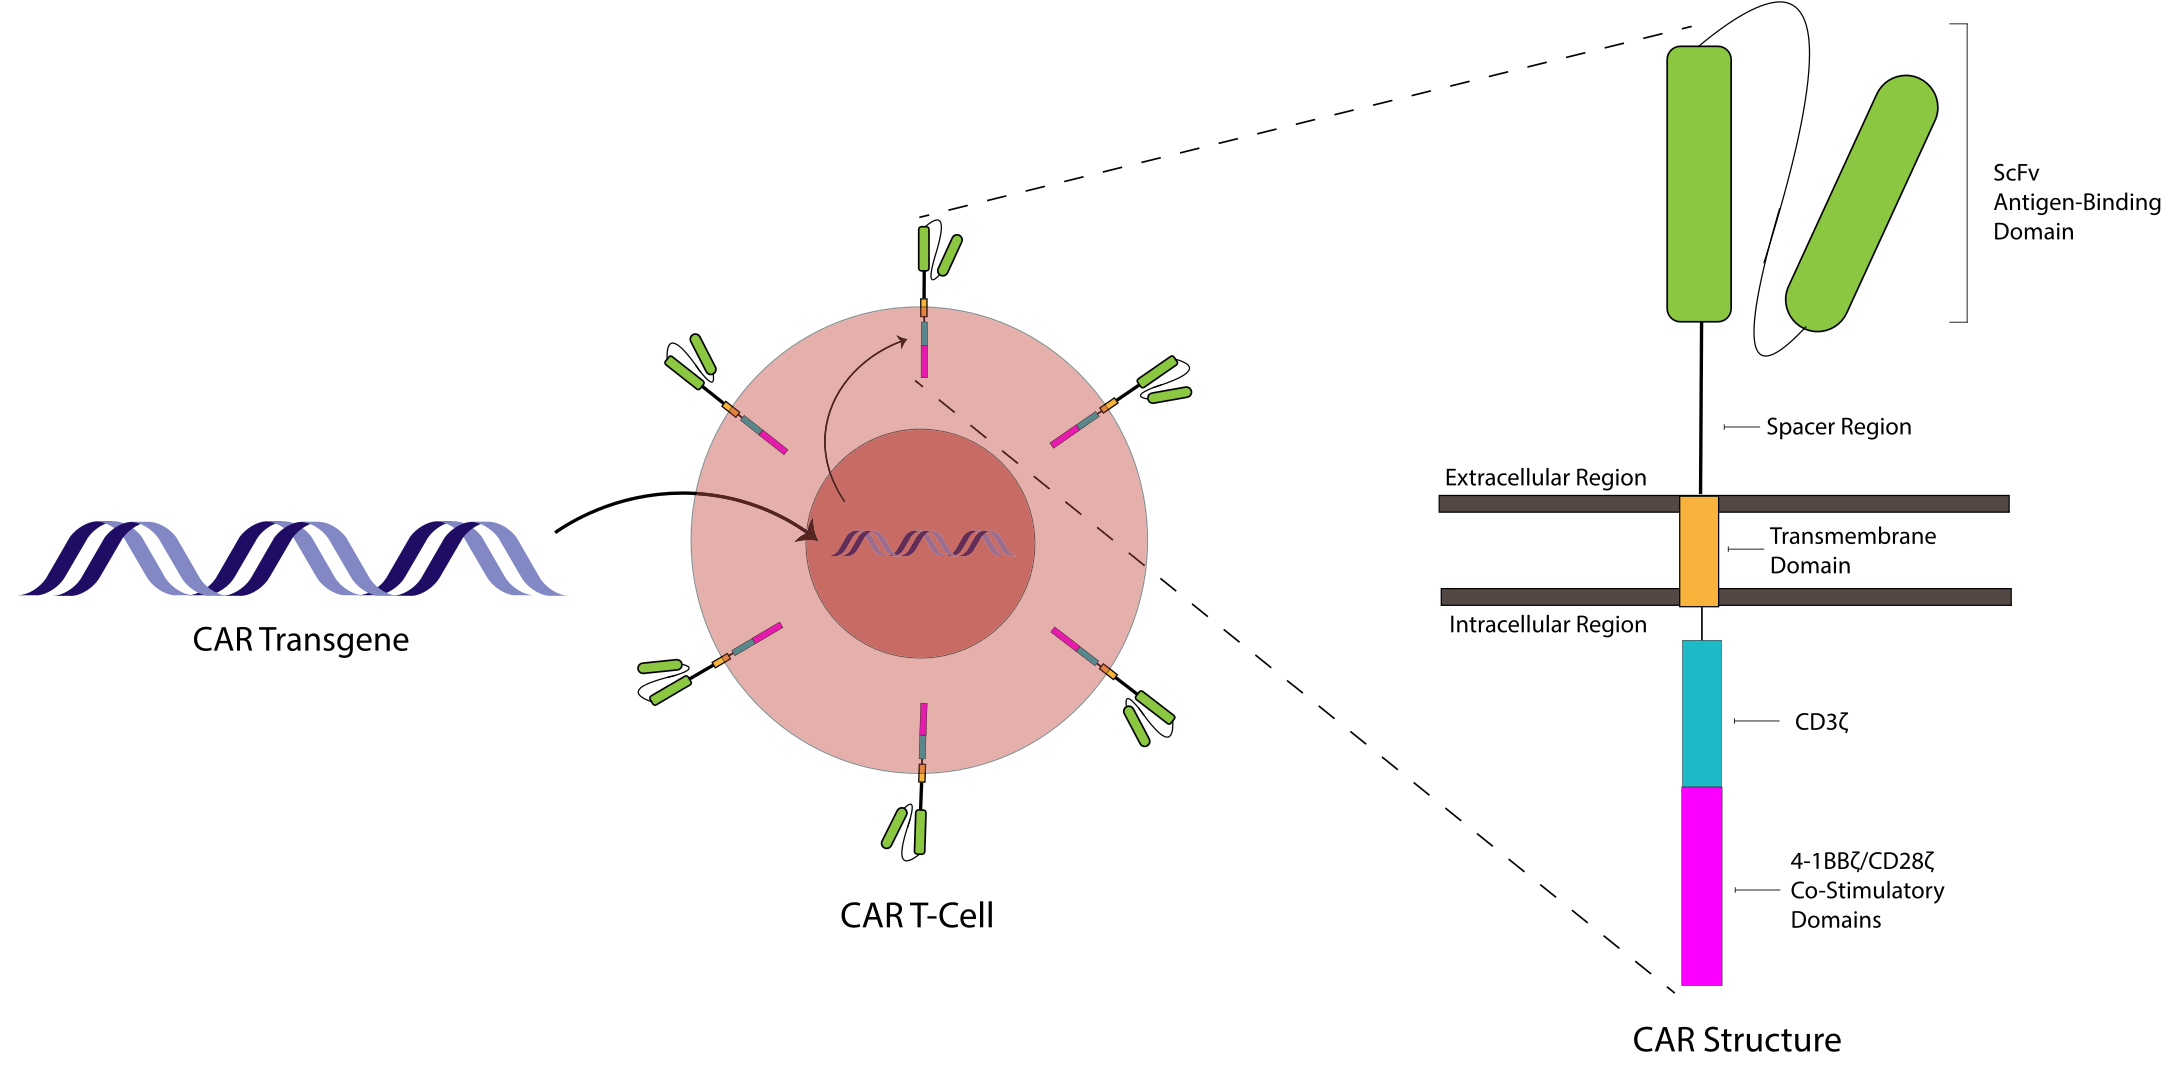
\includegraphics[width=0.7\textwidth]{cart.png}
    \caption{CAR-T细胞示意图}
    \label{cart}
\end{figure}
\par 然而，CAR-T细胞在临床治疗过程中可能面临一系列问题。因为该疗法本身基于体外的细胞培养和改造，基因编辑自然也成为其改进的称手工具。细胞疲劳(exhaustion)指癌症患者体内T细胞功能丧失，这使得CAR-T细胞无法完成靶向病灶的任务。通过CRISPR-Cas9可以敲除抑制CAR-T细胞功能的负调控分子(negative regulators)，例如PD-1、CTLA-4、LAG-3和TIM-3，这些基因的敲除能够减少T细胞疲劳，提高CAR-T细胞的持久性和杀伤力。还可以通过敲除二酰基甘油激酶（DGK）是的T细胞能够更好地抵抗肿瘤微环境中的免疫抑制因子。
\par T细胞在工作过程中会产生治疗所不希望的若干副作用，通过CRISPR-Cas9编辑，还可以精准调控细胞因子的表达，例如在CAR-T细胞中敲除GM-CSF和IL-6基因，从而减少细胞因子释放综合征（CRS）和神经毒性。而将IL-15基因整合到特定位点，使其受内源性启动子的调控，提供时间和空间上的表达控制，则可增强CAR-T细胞的持久性并减少系统性的副作用。
\par 除了通过敲除和整合基因以改善T细胞的性能外，CRISPR-Cas9还可以代替病毒载体将CAR基因\textbf{定点}插入T细胞受体$\alpha$链常量区（TRAC）位点。这种方法可以实现均一的CAR表达，避免因插入位置随机导致的功能差异。此外，结合多基因编辑（如敲除TRAC、PD-1和β-2微球蛋白基因），可以得到对免疫抑制更具抗性的“万能”CAR-T细胞。
\par 总结来说，以CRISPR-Cas9为首的现代基因编辑技术为遗传疾病和非遗传疾病的治疗都提供了强有力的分子级别的工程手段。前者有望通过胚胎基因编辑修正家族遗传的基因缺陷、以及通过靶向基因编辑改善基因病患者的症状甚至治愈之；后者得益于精准利用和改进人体细胞和免疫系统的能力，有望实现对癌症的有效治疗。尽管问题依然很多，但基因编辑技术的进步无疑是现代医学进步的有一个里程碑。


\bibliography{../MyLibrary}
\bibliographystyle{ieeetr}

\end{document}